\section{Overview}

\subsection{Motivation}
Plasmas, commonly called the fourth state of matter, are a gas where a
significant fraction of the neutral atoms or molecules have been split into
pairs of electrons and positive ions. Initially, a curiosity of the laboratory,
they have become a critical part of every day life. The electrically charged
nature of plasmas makes them a practical means by which to convert electrical
energy into electromagnetic, chemical, kinetic, or even nuclear energy. From an
applications perspective, they are indisposable in lighting, semiconductor
manufacturing, plastic processing, and space propulsion. On a more broad scale,
virtually all observable light in the universe is the result of a plasma in some
form or another \cite{NA2007}.

Some exceptions aside, only three things are required to create a plasma: a gas,
an energy source, and a means of transferring the energy to the gas. In man-made
applications, the energy source is typically electricity, and the simplest
transfer mechanism is via two electrodes placed on either side of the gas. The
application of a potential difference to these electrodes produces an electric
field as seen in figure~\ref{fig:avalanche}.
\begin{figure}
  \centering
  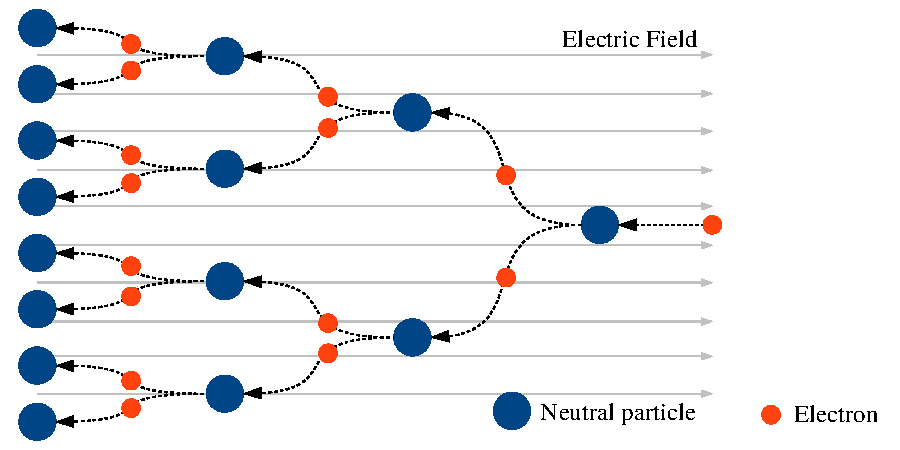
\includegraphics{./chapters/introduction/figures/avalanche.pdf}
  \caption{A simplified depiction of the avalanche breakdown process in a gas.}
  \label{fig:avalanche}
\end{figure}
The field accelerates a single seed electron in the gas (often created by
background cosmic radiation) until it collides with a neutral particle. The
electron, having acquired a sufficient amount of energy, liberates a second
electron loose from the particle, leaving behind a relatively heavy and immobile
ion. Subsequently, both the first and second electron are now accelerated by the
electric field. Again, they collide with two more neutral atoms, creating two
new electrons. As long as the electric field persists, the number of electron
and ion pairs increases exponentially. This process is generally referred to as
an avalanche.

Eventually, the production of ions and electrons in the gap balances out with
the rate at which they leave the system, whether by collection at the electrodes
or some other process. The resulting ionized gas may be referred to as a plasma
if it meets certain criteria. Simply put, there must be a high enough density
and number of charged particles for their electromagnetic interaction to
dominate over random collisions with neutral gas particles.

Despite this relatively simple recipe, the physical characteristics can vary
greatly depending on what gas is used, what pressure it is at, what voltage is
used, whether the electricity is applied constantly or varied over time, what
kind of electrodes are used, etc. As a result, man-made plasmas are generally
produced under very specific conditions. For example, a plasma etcher used in
semiconductor manufacturing may need to operate operate at pressures that are
one-thousandth of atmospheric pressure with ultra-pure (99.999\%) gases
\cite{Greenberg1993a}.

Plasmas like those which occur in plasma etchers, feature ions and neutral gas
particles with temperatures that are below 1,000 K, or roughly 1,340$^\cdot$ F.
Though this temperature is relatively high compared to room temperature, it is
well below the temperature of the electrons which may be in excess of 20,000 K.
Plasmas which exhibit this disparity in temperatures are often called
nonequilibrium or ``low-temperature'' plasmas.

Conversely, there exists another class of plasmas where the electrons, ions, and
neutral particles are all at the same temperature. These are called thermal
plasmas. Generally speaking, the closer the gas pressure is to atmosphere, the
more thermal a plasma is owing to the rapid increase in the frequency of
collisions between neutral and charged particles \cite{Kunhardt2000}.
Additionally, the temperatures in a thermal plasma can be quite high and, in
many cases, can easily melt all metals assuming that the total energy content of
the plasma is high enough. For example, the arc of an arc welder is a thermal
plasma. Similar high temperature plasmas, have a number of other applications
which include a variety of high-intensity lamps, metal cutting, and surface
coating.

There are, however, a number of applications which would benefit from operation
at higher pressures, but with low-temperature ions and neutrals so as to avoid
heat damage. This has spurred a substantial amount of research on nonequilibrium
atmospheric-pressure plasmas (\acs{app}s) in recent years \cite{Becker2005}.
Ideally, such a plasma could be generated at or near atmospheric pressure with
hot electrons, but minimal heating of surrounding gas. Though this field of
research is still relatively young, it has produced a variety of new plasmas and
capabilities. One of the more ubiquitous examples is use of plasmas to process
the surface of plastics so that ink can adhere. Separately, nonequilibrium
\acs{app}s are the technology which drives plasma televisions \cite{Rauf1999}.

As mentioned, these applications promise to be the first of many for such
plasmas. More recently, there have been innovative proposals to use these
plasmas in water purification \cite{Malik2001}, wound sterilization
\cite{Ayan2009}, improved combustion engines \cite{Nishihara2007}, nanoparticle
production \cite{Ostrikov2011}, and more. However, each situation has its own
challenges when it comes to the design and development of a plasma source,
particularly at these elevated pressures. Particularly problematic is the
tendency of \acs{app}s to develop instabilities which can cause them to rapidly
transition to thermal plasmas in a matter of nanoseconds.

There exist a few ways of getting around these instabilities. One example is the
dielectric-barrier discharge which passively regulates the amount of power which
can be deposited into the plasma \cite{Kogelschatz2003}. Another example
includes split-ring resonators which use natural feedback mechanisms to damp out
potential instabilities \cite{Iza2005}. The technique considered here, referred
to as the repetitively-pulsed nanosecond discharge, or \acs{rpnd}, uses high
voltage pulses which are so short that the instability does not have time to
develop \cite{Adamovich2008}. The \acs{rpnd} is a nonequilibrium plasma which
can operate at pressures ranging from approximately $10^{-3}$--$1$ atmospheres
\cite{Vasilyak1994}. At atmospheric pressure the \acs{rpnd} can produce a
uniform plasma in volumes on the order of 10 mL \cite{Walsh2006}. As the
pressure is reduced, the plasma volume can reach the order of liters
\cite{Starikovskaia1998}.

The importance of large-area, uniform, high-pressure plasmas such as the
\acs{rpnd} was highlighted in the National Academies' most recent decadal survey
of plasma science \cite{NA2007}. However, there is still much that is not know
about such plasmas. From the same survey, it is said that ``the full promise of
\acs{app}s will be known only if they can be understood and managed based on
fundamental scientific principles at two extremes--the nanoscopic kinetic level,
where selective chemistry occurs, and the global stability level.'' It is this
challenge, specifically the investigation of the nanoscopic kinetic level, which
drives the research presented here.

\subsection{History}

Historically, the study of low-temperature \acs{app}s has been almost
indistinguishable from the study of plasmas as a whole. However, this was not
necessarily a matter of reasoned choice. Plasma generation at
atmospheric-pressure obviates the need for an effective vacuum pump.
Additionally, prior to the creation of large battery banks, early sources of
electrical energy had relatively small capacities. This precluded the generation
of thermal atmospheric plasmas which required large amounts of energy.

Indeed, the requirements for a low-temperature \acs{app} are sufficiently
rudimentary that the first man-made one (and likely the first man-made plasma),
was probably a spark generated by rubbing fur against amber. This is commonly
attributed to Thales of Mil\^{e}tus from around 600 B.C. Following Thales,
electrical sparks came to intrigue many scientists including Gottfried Liebniz,
Benjamin Franklin, and Charles Wheatstone. By the mid-1800s, Pl\"{u}cker,
Gei\ss{}ler, and Hittorf began some of the first work on low-pressure plasmas
though it was Crookes who would later identify plasma as a separate state of
matter. Later, J.J.\ Thomson's discovery of the electron and discretized charge
in 1897 marked the beginning of modern plasma research.

By this time, the necessary tools and techniques existed to create steady
plasmas in pure, rarified gases. The behaviors of which were dominated by the
motion and interaction of the charged electrons and ions. Critically, the
effects of the neutral particles were negligible, thus isolating the electrical
properties of the plasma. These carefully controlled systems were ideal for
basic studies of plasma behavior and were used to great effect by individuals
such as Lewi Tonks and Irving Langmuir \cite{Tonks1929}. In fact, many modern
concepts in plasma physics can be traced back to their work.

In contrast, the pulsed \acs{app}s, characteristic of the earliest man-made
plasmas \cite{Anders2003}, were easy to create, but notoriously difficult to
work with. It could take them only a few nanoseconds to form, and less than a
millisecond to decay away. For many years, there were simply no instruments
capable of taking measurements this quickly. Furthermore, the neutral particles
which were of no consequence in the low-pressure plasmas, could not be ignored.
The neutral particles were present in such quantities that they could confound
or obscure otherwise simple measurements.

As a consequence, there is still a great deal that is not known about about
pulsed \acs{app}s, particularly lightning, streamers, and a type of plasma which
Thomson referred to as a ``luminous front.'' By the 1970s, this latter plasma
had come to be called the fast ionization wave, or \acs{fiw}
\cite{Vasilyak1994}. It was generated by a single voltage pulse lasting around
100 nanoseconds and peaking at 10s or 100s of kilovolts. For the right pressure
and gas, the \acs{fiw} could fill volumes of nearly 40 L with a relatively
uniform plasma, but with little heating of the gas.

These properties were attractive for a number of uses, but the \acs{fiw} faced a
number of implementation-related challenges. The switches used to trigger the
\acs{fiw} could only operate up to 100 times each second
\cite{Starikovskaia2001}. Unfortunately, the lifetime of a plasma at elevated
pressures is relatively short, and the plasma generated by the \acs{fiw} would
decay away quickly after each pulse. This meant that the \acs{fiw}-generated
plasma had a relatively low duty cycle; the ratio of the time the plasma spends
on to the time it spends off. This was disadvantageous for plasma-processing
applications where low duty cycles are equivalent to long processing times. The
low duty cycle also necessitated so-called preionization of the gas with UV
lamps or a secondary plasma generator, adding to the cost and complexity of the
system \cite{Levatter1980}. Finally, the pulse generators used for \acs{fiw}s
were not considered reliable enough for long operational lifetimes.

Recent advances in solid-state switching technology has largely solved these
issues. At present, switches exist which can reliably operate 100,00 times a
second; sufficiently fast that the plasma duty cycle approaches 100\%
\cite{Efanov1997}. This has the additional benefit of obviating the need for a
preionization stage, as a sufficient number of electrons persist between pulses.
The discharge produced by the use of these new switches is what we refer to as
the \acs{rpnd}.

\subsection{Questions}

The large pedigree of pulsed plasma research belies the fact that they are still
not well-understood. This remains especially true for \acs{rpnd}s which present
significant experimental challenges. A major component of this has to do with
the time scales associated with the \acs{rpnd}. The formation of a \acs{rpnd}
often requires no more than a few nanoseconds. Very sensitive equipment is
required in order to measure changes which occur during this period.
Unfortunately, such equipment is particularly susceptible to the broadband
electronic noise generated by both real and displacement currents of the fast
pulses. There is a plethora of other problems that can be traced back to topic
of timing. For example, the length and insulators of detector cables can
introduce substantial delays, and must be considered in order to synchronize
different measurements.

Consequently, the majority of \acs{rpnd} studies focus on measurements after the
discharge has occurred, when changes happen at a much slower rate. A great deal
of information is available for this period of time, including chemical
compositions, atomic densities, electron densities, gas temperatures, and more.
While undoubtedly important, these measurements provide limited insight on what
is happening \emph{while} the plasma is forming. It is natural, then, to ask,
what are the \acs{rpnd} plasma properties during formation?

Additionally, most studies have used a limited range of gases: oxygen, nitrogen,
air, hydrogen, or some mixture thereof. The choice of these gases is deliberate
and reflects specific applications in combustion and aerospace. However, the use
of rare gases (such as helium) and rare gas mixtures has become popular because
they provide for a wider range of stable operating conditions. Notably, it has
been found that the unique internal electronic structure of rare gases can
produce very different discharges. Given this, there is the question of how rare
gas \acs{rpnd}s compare to more conventional ones.

Finally, the persistence of the plasma between pulses makes the development of a
\acs{rpnd} very different from a \acs{fiw}.

Finally, though the \acs{rpnd} and \acs{fiw} are qualitatively similar, there
are some fundamental differences between the two. These largely stem from the
persistence of the plasma between pulses. It is this plasma which guarantees
uniform breakdown in the case of \acs{rpnd}, while the \acs{fiw} is largely
dependent on very high energy electrons. At the same time, if the plasma is too
dense at the beginning of the voltage pulse, it can limit the final density of
the electrons and excited atoms. Because plasma-induced chemistry is a product
of these particles, this pre-pulse plasma plays a decisive role in the number of
reactions a \acs{rpnd} can produce. Therefore, one must ask how the properties
of a \acs{rpnd} compare to those of a \acs{fiw} and how they vary with the
operating conditions.

\subsection{Approach}

The dissertation presented here represents efforts to either answer or provide a
foundation to answer these questions. In order to develop the appropriate
context for this work, the next section will be a comprehensive review of the
\acs{rpnd} literature. It begins with the first reported pulsed \acs{app}s and
concludes with contemporary studies.

The following two chapters set the basis for the experimental and numerical
studies. Chapter~\ref{chp:theory} presents the theory necessary to understand
\acs{rpnd}s including streamer discharges, atomic spectroscopy, and collision
processes. Subsequently, Chapter~\ref{chp:experiment} describes the design of
the helium \acs{rpnd} discharge apparatus used for the experimental studies and
as the basis for the simulations. Also included in this chapter are several
measurements of the basic discharge properties.

Chapters~\ref{chp:metastables} through~\ref{chp:modeling} provide more detailed
measurements and analysis of the \acs{rpnd} dynamics. In
Chapter~\ref{chp:metastables}, the measurements of the helium metastables in a
\acs{rpnd} are presented and analyzed as a function of pressure an axial
location in the discharge apparatus. Chapter~\ref{chp:emissions} presents and
analyzes similar measurements of the spontaneous plasma emissions. Finally,
Chapter~\ref{chp:modeling} discusses the development of a global model for a
helium plasma and its use with the experimental data to infer the plasma
properties of the \acs{rpnd}. The dissertation concludes with a summary of the
results and suggestions for further avenues of research.

\section{Literature Review}

\acs{rpnd}s are only a recent invention which resulted from advances in
fast-switching semiconductors. However, the physics of their formation is
related to a much more broad category of plasmas which includes lightning,
streamers, and even some transient phenomena in DC glows \cite{Loeb1965}. These
plasmas are unique in that their spatial structure develops at speeds much
faster than can be accounted for by the conventional Townsend mechanism. Loeb
refers to this phenomena as ``ionizing waves of potential gradient.''\footnote{It 
should be noted that the phrase wave does not indicate any kind of
periodic motion or spatial arrangement. Simply put, it describes a boundary
which separates ionized and unionized gas which travels from one electrode to
another.}.

\subsection{Early History of Pulsed Discharges}

In 1835 (as reported by Thomson \cite{Thomson1893}), Charles Wheatstone
attempted to measure what he thought to be the speed of electricity in a
six-foot long discharge tube of unspecified pressure \cite{Wheatstone1835}. It
is now known that he was actually measuring the speed with which a plasma formed
between the two electrodes. He accomplished this by the use of a rotating mirror
which allowed him to see images of two sections of the tube, slightly displaced.
The displacement between the images was proportional to the speed with which the
plasma traveled between them. Wheatstone estimated this speed to be at least
$8\times10^7$ cm/s.

Interestingly, von Zahn later noted that this was \emph{not} the speed of the
emitting particles \cite{Zahn1879}. The visible light did cross the gap at an
appreciable speed, but there was no detectable Doppler shift in the light
emitted parallel to the propagation. As a result, it was concluded the
light-emitting particles could not be traveling at the same speed as the light.

Later, Thomson revisited this work with an improved apparatus
\cite{Thomson1893}. This included a tube that was now 15 m in length and five mm
in diameter, as seen in figure~\ref{fig:thomson}.
\begin{figure}
  \centering
  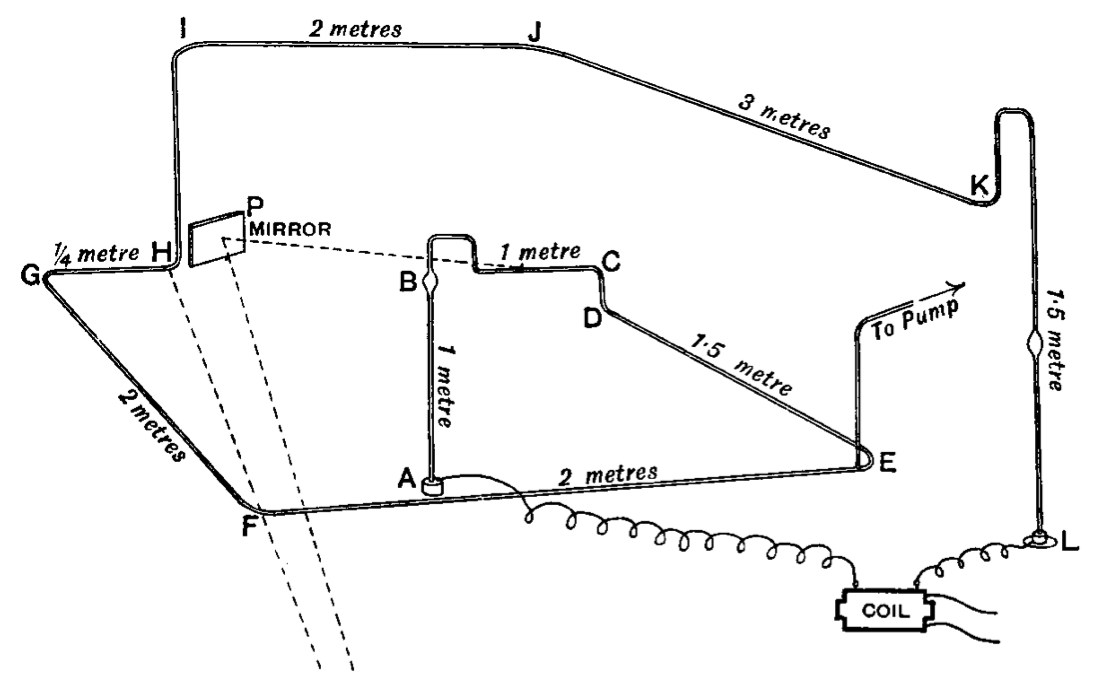
\includegraphics[width=4in]{chapters/introduction/figures/thomson.png}
  \caption{A sketch of J.J. Thomson's early experiments on pulsed plasmas 
  in long vacuum tubes \cite{Thomson1893}.}\label{fig:thomson}
\end{figure}
Also using the rotating mirror apparatus, Thomson was able to greatly improve on
the estimates of Wheatstone. He estimated that the so-called ``luminous front''
had a speed that was more than $1.5\times10^{10}$ cm/s, or in excess of half of
the speed of light. Furthermore, Thomson determined that the luminous front
always appeared to travel from the positively pulsed electrode (anode) to the
ground electrode (cathode).

The study of these luminous fronts was revisited by several researchers in the
wake of Thomson \cite{James1904, Whiddington1925, Beams1926}, but their attempts
to duplicate the measured speeds were met with varied success. In 1930, Beams
confirmed definitively confirmed those of Thomson. He also found that the front
always initiated at the electrode with the highest, absolute potential, relative
to ground. Beams hypothesized that the rapid motion of the front was a result of
a self-propagating region of high space charge, quote:
\begin{quote}
  In the neighborhood of the electrode $\ldots$ the field is very high and
  intense ionization should take place. This ionization due to the large
  difference in mobilities of positive ions, negative ions and electrons
  respectively should result in the establishment of a space charge. This space
  charge, once formed near the high potential electrode $\ldots$ must move
  down the tube regardless of the polarity of the applied potential because of
  the changes it produces in the field near its edges.
\end{quote}

At about the same time, Schonland and Collens reported on their observations of
lightning \cite{Schonland1933}. Though the general structure and length scale of
lightning is substantially different from the luminous fronts observed by Beams
and Thomson, the two phenomena would later prove to be very similar. In their
work Schonland and Collens noted that lightning would usually occur in a
two-step process. Based on the images they obtained, they suggested that
the leader was generated by a relatively small ``dart'' with a mean vertical
velocity of $7.2\times10^8$ cm/s. The dart moved in a random manner, changing
directions at random intervals, but always moving toward the ground.

The second step began when this dart reached the ground. Once there, a bright
return stroke would occur along the same path that the leader had traced out. In
contrast to the leader stroke, the return stroke had a velocity of $5\times10^9$
cm/s. Schonland and Collens hesitantly attributed the leader stroke to an
extended electron avalanche, and the return stroke to thermal ionization along
the conductive path generated by the dart. However, calculations by Cravath and
Loeb showed that the speeds of the proposed avalanche was inconsistent with the
fields at the head of a lightning stroke \cite{Cravath1935}. Instead, they
suggested that the dart was actually a moving region of space charge which
locally accelerated electrons to ionizing energies. This was similar to the
mechanism earlier proposed by Beams.

\subsection{The Streamer Model}

It was long known that sparks in air were similar to lightning. Advances in
technology during the 1930's led to experiments which reinforced this
similarity. In response to the measurements of Schonland and Collens; Snoddy,
Beams, and Dietrich studied the breakdown of gas in a long tube with both
positive and negative applied potentials \cite{Snoddy1936}. Using an
oscillograph, they observed both the leader and a return stroke in both cases.
However, the propagation of the plasma wave toward the cathode required a source
electrons ahead of the wave. The authors proposed that photoionization might
provide these necessary electrons.

Around the same time, Flegler and Raether had come to a similar conclusion
regarding the importance of photoionization. This led them to develop a more
thorough theoretical model for these waves \cite{Flegler1936} which came to be
known as the streamer theory. This was followed by a similar treatment by Loeb
and Meek \cite{Loeb1940, Loeb1940a, Meek1940}. The streamer theory divided the
initial plasma formation into two steps. In the first step, an electron
avalanche is initiated between two electrodes. The avalanche travels toward the
anode and leaves behind a region of positive space charge. In the second step,
the return stroke begins at the anode and travels along the conductive path
generated by the initial avalanche toward the cathode.

The streamer model proved relatively successful in describing the development of
sparks and lightning. Theoretical estimates of the speed matched the velocity
measurements that were acquired with photographs and oscillographs.
Additionally, the theory was able to account for the branching manner in which
lightning was formed as well as the constriction in space.

Following the initial work of Flegler, Raether, Loeb, and Meek, a number of
researchers began to explore the boundary between the Townsend mechanism and the
streamer mechanism. Most notable was Fisher and Bederson's work in 1951
\cite{Fisher1951}, which was later extended to nitrogen \cite{Kachickas1952} and
argon \cite{Kachickas1953}. These studies suggested that the streamer theory was
incomplete. Furthermore, the reliance of the streamer theory on photoionization
would later prove very contentious \cite{Kunhardt1988}. Finally, there was a
whole class of discharges that it did not readily explain.

\subsection{Diffuse Streamers}

As noted by Chalmers \cite{Chalmers1971}, Rogowski and Buss \cite{Rogowski1927,
Buss1932} observed a fast, diffuse, glow discharge immediately prior to the
filaments of a streamer discharge. Allibone and Meek, noted similar diffuse
discharges in air based on oscillographs and photographs \cite{Allibone1938,
Allibone1938b, Allibone1938c}. However, the Boys apparatus \cite{Boys1926} which
was employed in these studies (an ancestor to the modern streak camera) was
unable to capture the evolution of the diffuse glow, given its large spatial
extent.

This was first noted by Allibone who attempted to use Lichtenberg
figures\footnote{Such figures directly exposed photographic emulsions to the
electrical discharge. The developed image was a time-integrated representation
of the discharge.} to definitively capture this diffuse glow
\cite{Allibone1948}. Later, Saxe and Meek used the recently invented
photomultiplier tube to record the evolution of the light emissions in the
brief, diffuse glow \cite{Saxe1948} as a function of space. Both studies
agreed in the existence of the diffuse glow, despite some disagreement on the
nature of its geometry and propagation.

By 1968 (according to Kunhardt and Byszewski \cite{Kunhardt1980}), Stankevich
and Kalinin had provided the most firm evidence yet of a diffuse discharge in a
dense gas \cite{Stankevich1968}. This was later confirmed by experiments with a
pulsed nanosecond discharge by Mesyats, Bychkov, and Kremnev \cite{Mesyats1972}.
In their analysis, they concluded that photoionization could not play a role in
such short-lived discharges. The formation of their discharge only required
several nanoseconds, much shorter than the lifetimes of the excited states
responsible for photon emission. They suggested that the streamer model required
some extension.

In addition to the diffuse discharge, Stankevich and Kalinin also noted the
detection of x-rays with each pulse. This suggested the presence of high-energy
electrons impinging on the surface of the electrodes, despite the high
collisionality of the dense gas. Not only that, but the electron energies could
even exceed what would be expected from the vacuum electric fields
\cite{Babich1977}. The eventual conclusion was that the electric field
associated with the space charge at the head of the streamer produced very
energetic electrons which deposited their energy far from the streamer tip
\cite{Kunhardt1980, Babich1990}, allowing the streamer to spread out beyond the
diffusive region of the electrons.

It was based on the studies of the fast electrons in these discharges that
Mesyats, Bychov, and Kremnev proposed the use of a fast electron beam for
pumping high-pressure gas lasers. Similar work was conducted simultaneously by
Fenstermacher et al.~\cite{Fenstermacher1972}. Palmer \cite{Palmer1974}, and
Levatter and Lin \cite{Levatter1980} determined that there was a threshold
amount of preionization required to ensure homogeneity of the discharge. Hunter
\cite{Hunter1976}, and Koval'chuk and Mesyats \cite{Koval'chuk1976} later
proposed that such discharges be used for fast-closing switches. Gas lasers and
fast switches would drive much of the later research on fast, pulsed discharges.

Eventually these discharges came to be referred to as fast ionization waves
(\acs{fiw}s). A large body of Russian literature developed around their study,
though much of it has remained untranslated. In 1994, Vasilyak produced an
extensive review of these studies \cite{Vasilyak1994}. The data include wave
velocities for a variety of gases and pressures. Other parameters such as
attenuation coefficients for the waves, high energy electron currents, electric
field measurements, and a circuit model of the \acs{fiw} are also included.

\subsection{Repetitively-Pulsed Nanosecond Discharges}

The type of discharge originally studied by Babich, Loika, and Tarasova came to
be known as the fast ionization wave (\acs{fiw}). In the years following its
discovery, a substantial effort was made to document the properties of the
\acs{fiw} over a wide range of conditions. In these studies, the wave velocity,
current, and attenuation were the most frequently measured quantities. Much of
this work is summarized in a review by Vasilyak \cite{Vasilyak1994}. Also
reviewed are Slavin and Sopin's work which was the first to attempt a
computation of the electron energy distribution function \acs{eedf} in
\acs{fiw}s \cite{Slavin1992}.

The experimental measurements and computational work reported by Vasilyak were
expanded on by a series of studies conducted at the Moscow Institute of Physics.
These are reviewed by Starikovskaia et al.~\cite{Starikovskaia2001} and included
measurements of the electron density, electric field, and energy coupling for
\acs{fiw}s in air, nitrogen, and hydrogen. The computational work by
Starikoskaia and Starikovskii \cite{Starikovskaia2001a} still represents the
most detailed study of the \acs{eedf} in nitrogen \acs{fiw}s.

However, Starikovskaia et al.\ noted that the usefulness of \acs{fiw}s were
limited, in part, by their repetition rates. The power supplies for \acs{fiw}s
were capacitor banks, charged in parallel, and discharged in series (also
referred to Marx banks). Unfortunately, the spark gaps used to trigger these
capacitor banks would not operate above a few hundred Hz. This changed in the
late 1990's with the development and commercialization of fast, solid-state
switches. Specifically, with the fast ionization dynistor it was possible to
achieve repetition rates of 100 kHz \cite{Efanov1997}.

This led to a new class of repetitively-pulsed discharges, or the \acs{rpnd}.
These discharges operated at sufficiently high rates such that the electrons and
ions would persist in significant quantities between pulses. This meant that the
plasma duty cycle was increased by a significant amount. These improved
qualities of the \acs{rpnd} over the \acs{fiw} inspired a number of novel,
application-driven studies. This included:
\begin{itemize}
  \item Plasma-assisted combustion \cite{Pancheshnyi2006, Starikovskaia2006, 
        Adamovich2008}
  \item Magnetohydrodynamic energy bypass engines \cite{Macheret2002,
        Adamovich2008, Schneider2009a}
  \item Plasma actuators \cite{Starikovskii2009, Adamovich2009}
  \item High-pressure xenon lamps \cite{Nikandrov2008}
  \item Plasma medicine \cite{Ayan2009, Zimmermann2012}
  \item Water treatment \cite{Foster2013}
\end{itemize}
Though not specific to the \acs{rpnd}, Becker et al. \cite{Becker2005} provide
an extensive discussion of the potential uses for non-equilibrium air plasmas.

As a result, contemporary researchers have produced a wealth of literature on
the operation of \acs{rpnd}s. More recently, there have been detailed
measurements of the gas temperatures \cite{Pilla2006, Pancheshnyi2006,
Nishihara2006, Bao2007, Lou2007, Pai2009, Zuzeek2010, Nishihara2011}, chemical
composition \cite{Bao2007, Lou2007, Pai2009}, electric fields \cite{Ito2009,
Ito2010, Muller2011a}, and energy coupling \cite{Macheret2006, Pancheshnyi2006}.
Notably, these studies have been generally restricted to molecular gases; air,
nitrogen, and occasionally, hydrogen.

The first such study was the work of Laroussi and Lu who examined a \acs{rpnd}
excited in a stream of helium flowing from a tube into air \cite{Laroussi2005,
Lu2006}. The resulting plasma had the appearance of a jet, emitted from the open
end of the tube. Using fast photography they observed that the jet was actually
a series of plasma ``bullets'' formed with each pulse. Measurements of the
bullet velocities showed that their speed greatly exceed what would be expected
purely from electrons drifting under the applied electric field. They described
the bullet as a classic cathode-directed streamer propagated by photoionization.

The plasma bullets of Laroussi and Lu spawned a great deal of interest in
\acs{rpnd} helium plasma jets\footnote{A distinction should be made between
plasma jets, excited by sinusoidal power supplies, similar to the well-known
dielectric-barrier discharge \cite{Kogelschatz2003}, and those produced by
nanosecond pulses. Differences between the two were reported by Walsh, Shi, and
Kong \cite{Walsh2006}.} For example, Walsh et al.\ studied the atomic oxygen
production for helium-oxygen mixtures with the use of emission spectroscopy and
a global plasma chemistry model \cite{Walsh2010}. Urabe et al.\ employed a
variety of laser diagnostics to measure the radial density profiles of helium
metastable atoms and molecular nitrogen ions in a similar jet. This work was
supported by a number of two-dimensional plasma simulations such as those by
Naidis \cite{Naidis2010} and Breden, Miki, and Raja \cite{Breden2011}.

Simultaneously, there has been a decline in the study of \acs{fiw}s, and
relatively little on large-volume \acs{rpnd}s. One of the most recent \acs{fiw}
studies was produced by Takashima et al. \cite{Takashima2011}. In it, the
authors reported on \acs{fiw}s in helium and nitrogen which were studied using
capacitive probes and voltage-current characteristics. The results were compared
to extensive two-dimensional fluid simulations and an analytic, one-dimensional
drift model. In most cases, the measurements and simulations showed good
agreement.

\section{Summary}

Contemporary \acs{rpnd} studies have mostly focused on measurements in the
afterglow plasma or of time-integrated quantities. This has limited the
understanding of how \acs{rpnd}s develop as only so much can be inferred from
these measurements. Particular issues, such as the electron energetics in the
wave front are not firmly known. Relatedly, the relative importance of
photoionization and nonlocal electrons is still under debate. Even measurements
of common plasma parameters such as electron densities and temperatures are in
short supply. Each of these issues is important in the development of a thorough
theoretical understanding of \acs{rpnd}s, as well as the validation of
simulations, and optimization for real world applications.

Relatedly, the study of \acs{rpnd}s has generally been limited to molecular
gases such as air, nitrogen, oxygen, or combustion-related mixtures.
Consequently, little information has been published on rare gas \acs{rpnd}s, in
spite of the fact that their unique physics makes them ideal for certain uses.
For example, rare gas discharges exhibit very little gas heating, making them
desirable for the treatment of highly sensitive materials. Additionally, the
radiative emissions of rare gases have a range of uses from commercial lighting
to gas lasers. Finally, the large degree of Penning ionization resulting from
rare gases may make them useful in \acs{rpnd} gas mixtures as a means of
optimizing discharge properties.

In order to address these issues, this work will use a combination of
experiments and modeling to examine the plasma dynamics of a helium \acs{rpnd}
on time scales ranging from 5 ns to 100 $\mu$s and at pressures from 0.3 to 16.0
Torr. The nanosecond time scale results will be one of a very few datasets
available on the evolution of the \acs{rpnd} during its formation. This will
provide new insight on the dominant physical processes in the wave front. To
complement this, the microsecond time scale measurements will reveal the
dominant loss mechanisms in between pulses as well as the time-averaged
characteristics of the \acs{rpnd}. Lastly, the parameterization with pressure
will offer the chance to examine how the physics of the discharge is altered by
the collisionality.

Experimentally, the \acs{rpnd} will be studied by its current and voltage
characteristics, optical emissions, and with laser absorption spectroscopy. The
current and voltage characteristics will be used to determine the energy
absorbed by the plasma with each pulse. The optical emissions will provide
information about the excited state dynamics and the wave velocity. Finally, the
laser absorption spectroscopy will be used to resolve the short time scale
dynamics and as a benchmark for the numerical modeling. The modeling will focus
on the development of a detailed global model of a helium discharge. This model
will be informed by additional particle-in-cell simulations, and solutions of
the Boltzmann equation. Using the metastable measurements as a baseline, the
global model will be used to predict the electric field, electron temperature,
electron density, excited state densities, and emissions of the \acs{rpnd}.
